\section{Experiment Design}

To ensure experimental validity, all intermediate evaluation and hyperparameter tuning was performed on $23$ randomly selected images that were separate from both training image set of $106$ images and the final test set of $23$ images. All examples and images are taken from the evaluation set, with final metrics being taken on the test set. No results are taken from the train set, as they would have little meaning.

\section{Existing Pipelines}

To attempt to generate a baseline to assess new methods against, Tesseract \cite{SmithTesseract}, a popular OCR engine sponsored by Google \cite{Vincent} and Ocular \cite{Berg-Kirkpatrick}, another OCR engine based on stochastic models, were integrated into the pipeline using pytesseract \cite{Lee} and by calling jar files from python respectively.

\subsection{Evaluation Metrics}
\todo{NEW}

As these existing pipelines were assessed in the early phases of the project, a full ground truth to evaluate them on was not yet generated as the bounding of lines was not fully implemented. Therefore, they were assessed on how well they were able to detect the quantity of glyphs in an image and how visually close the transcriptions looked when the images were looked at by a human. These metrics proved to be enough to evaluate the methods as both methods were far enough away from an acceptable solution that a more exact metric for comparison was not needed.

\subsection{Tesseract}
\todo{NEW}

With Tesseract, using the ancient Greek corpus, and using both raw and binarized images, the output was comparable to noise, with the transcription lengths being an order of magnitude different from the ground truths.

\subsection{Ocular}
\todo{NEW}

Similarly, training Ocular on both raw and binarized full images and individual glyph images, the output was comparable to noise, with the transcription lengths being an order of magnitude different from the ground truths and each glyph being an alpha or lambda more than $95\%$ of the time regardless of the dataset that Ocular was trained on.

\section{Binarization}

\subsection{Evaluation Metrics}
\todo{NEW}

As there was no ground-truth information provided to compare binarizations against, visual comparison was utilized to determine which binarization method was providing the highest quality binarizations. This was done on four different images, which contained various features that would allow for quick visual evidence of the effectiveness of the methods \seefig{binarizationRaw}. The four images are of assorted sizes, from different collections, and are degraded to different degrees, allowing them to function as a valuable quick assessment tool without introducing bias into the evaluation of the methods.

To assess each binarization method, these images were used to determine how much of the ink on the papyrus was being included, and if noise was being added to the image in the form of background pixels being black or ink pixels being white. This metric was designed to ensure that the signal-to-noise ratio would be low and that the recall and precision would be high, even if they were not directly measurable without a ground truth for each pixel.

\begin{figure}
    \caption{Four Images Utilized to Visually Assess Binarization Quality}
    \label{fig:binarizationRaw}
    \begin{center}
        \begin{subfigure}[b]{0.45\textwidth}
            \centering
            \caption{Example File A}
            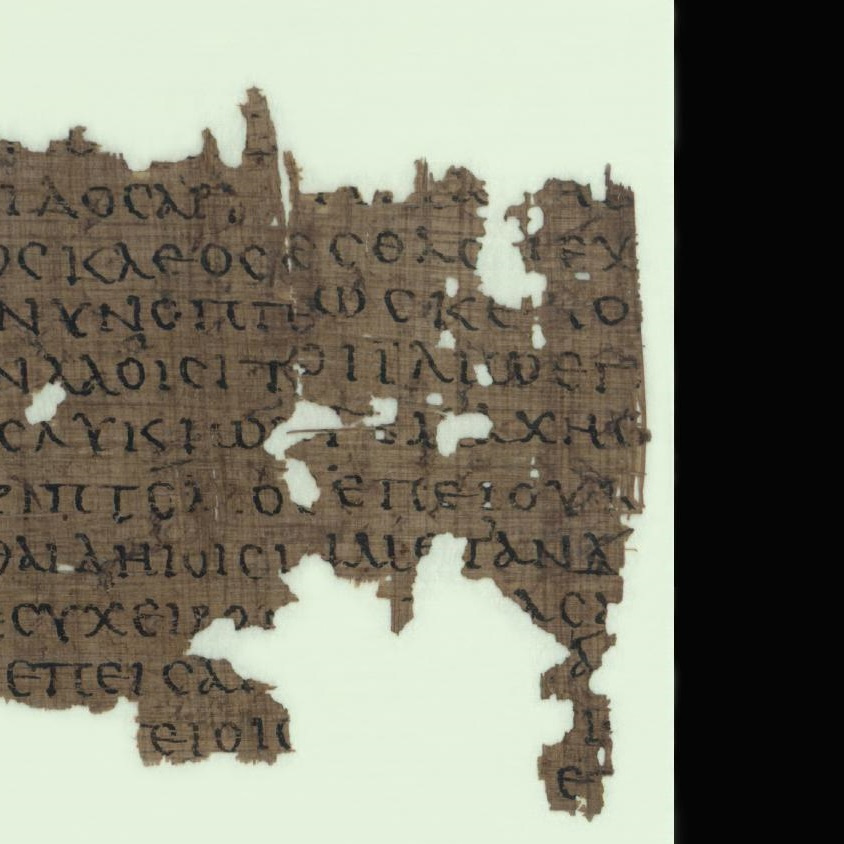
\includegraphics[width=\textwidth]{{raw/G_02317_26742_Pap_crop.jpg}}
        \end{subfigure}
        \hfill
        \begin{subfigure}[b]{0.45\textwidth}
            \centering
            \caption{Example File B}
            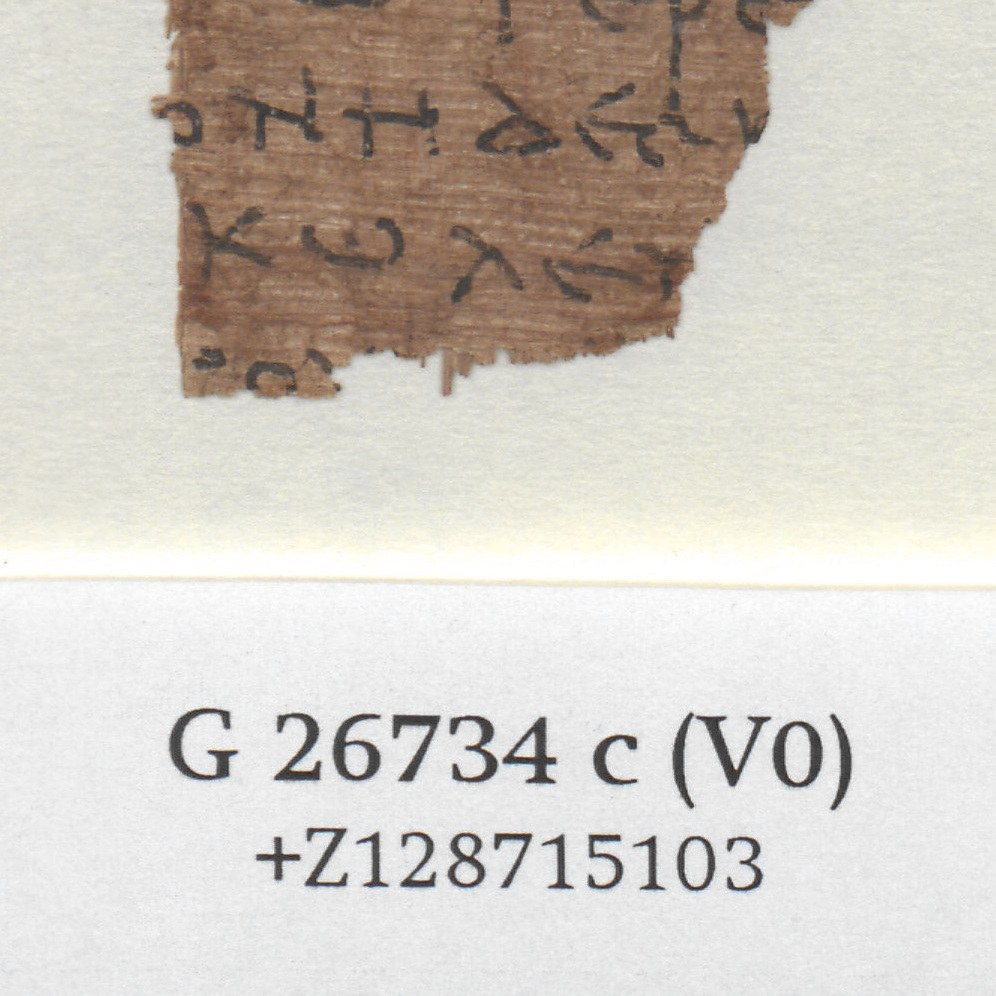
\includegraphics[width=\textwidth]{{raw/G_26734_c_crop.jpg}}
        \end{subfigure}
        \vfill
        \begin{subfigure}[b]{0.45\textwidth}
            \centering
            \caption{Example File C}
            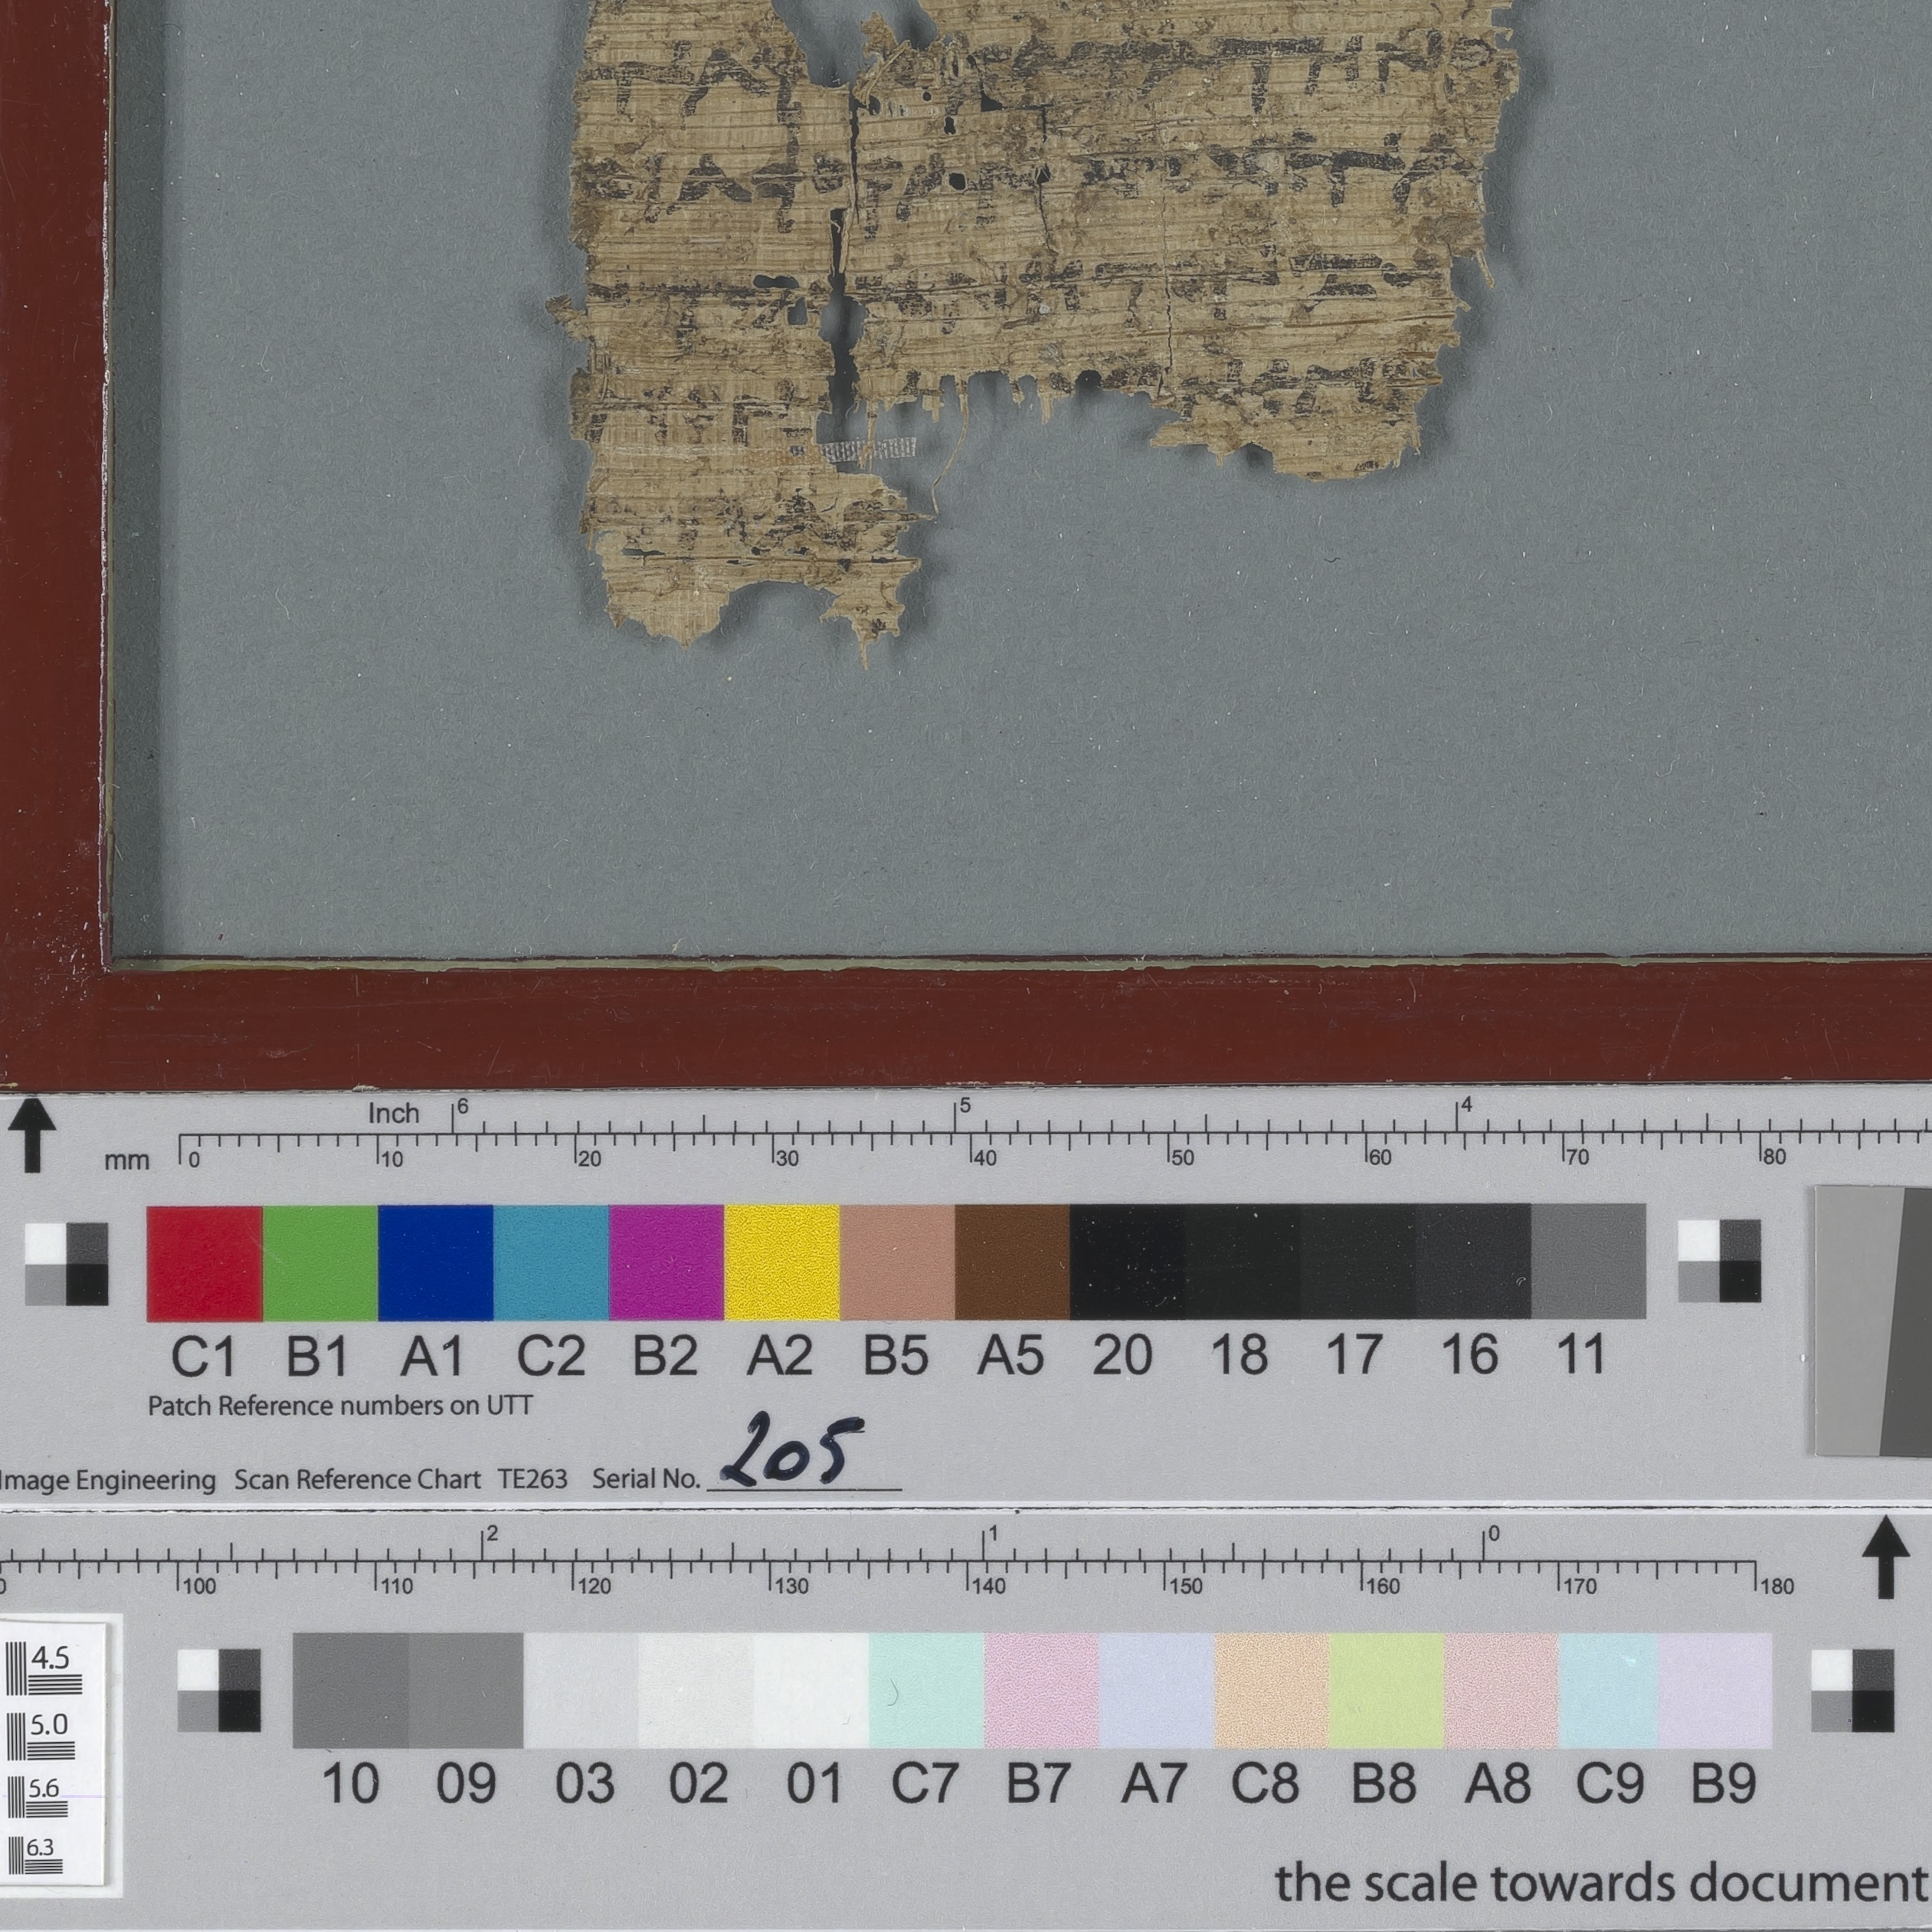
\includegraphics[width=\textwidth]{{raw/P_Hamb_graec_665_crop.jpg}}
        \end{subfigure}
        \hfill
        \begin{subfigure}[b]{0.45\textwidth}
            \centering
            \caption{Example File D}
            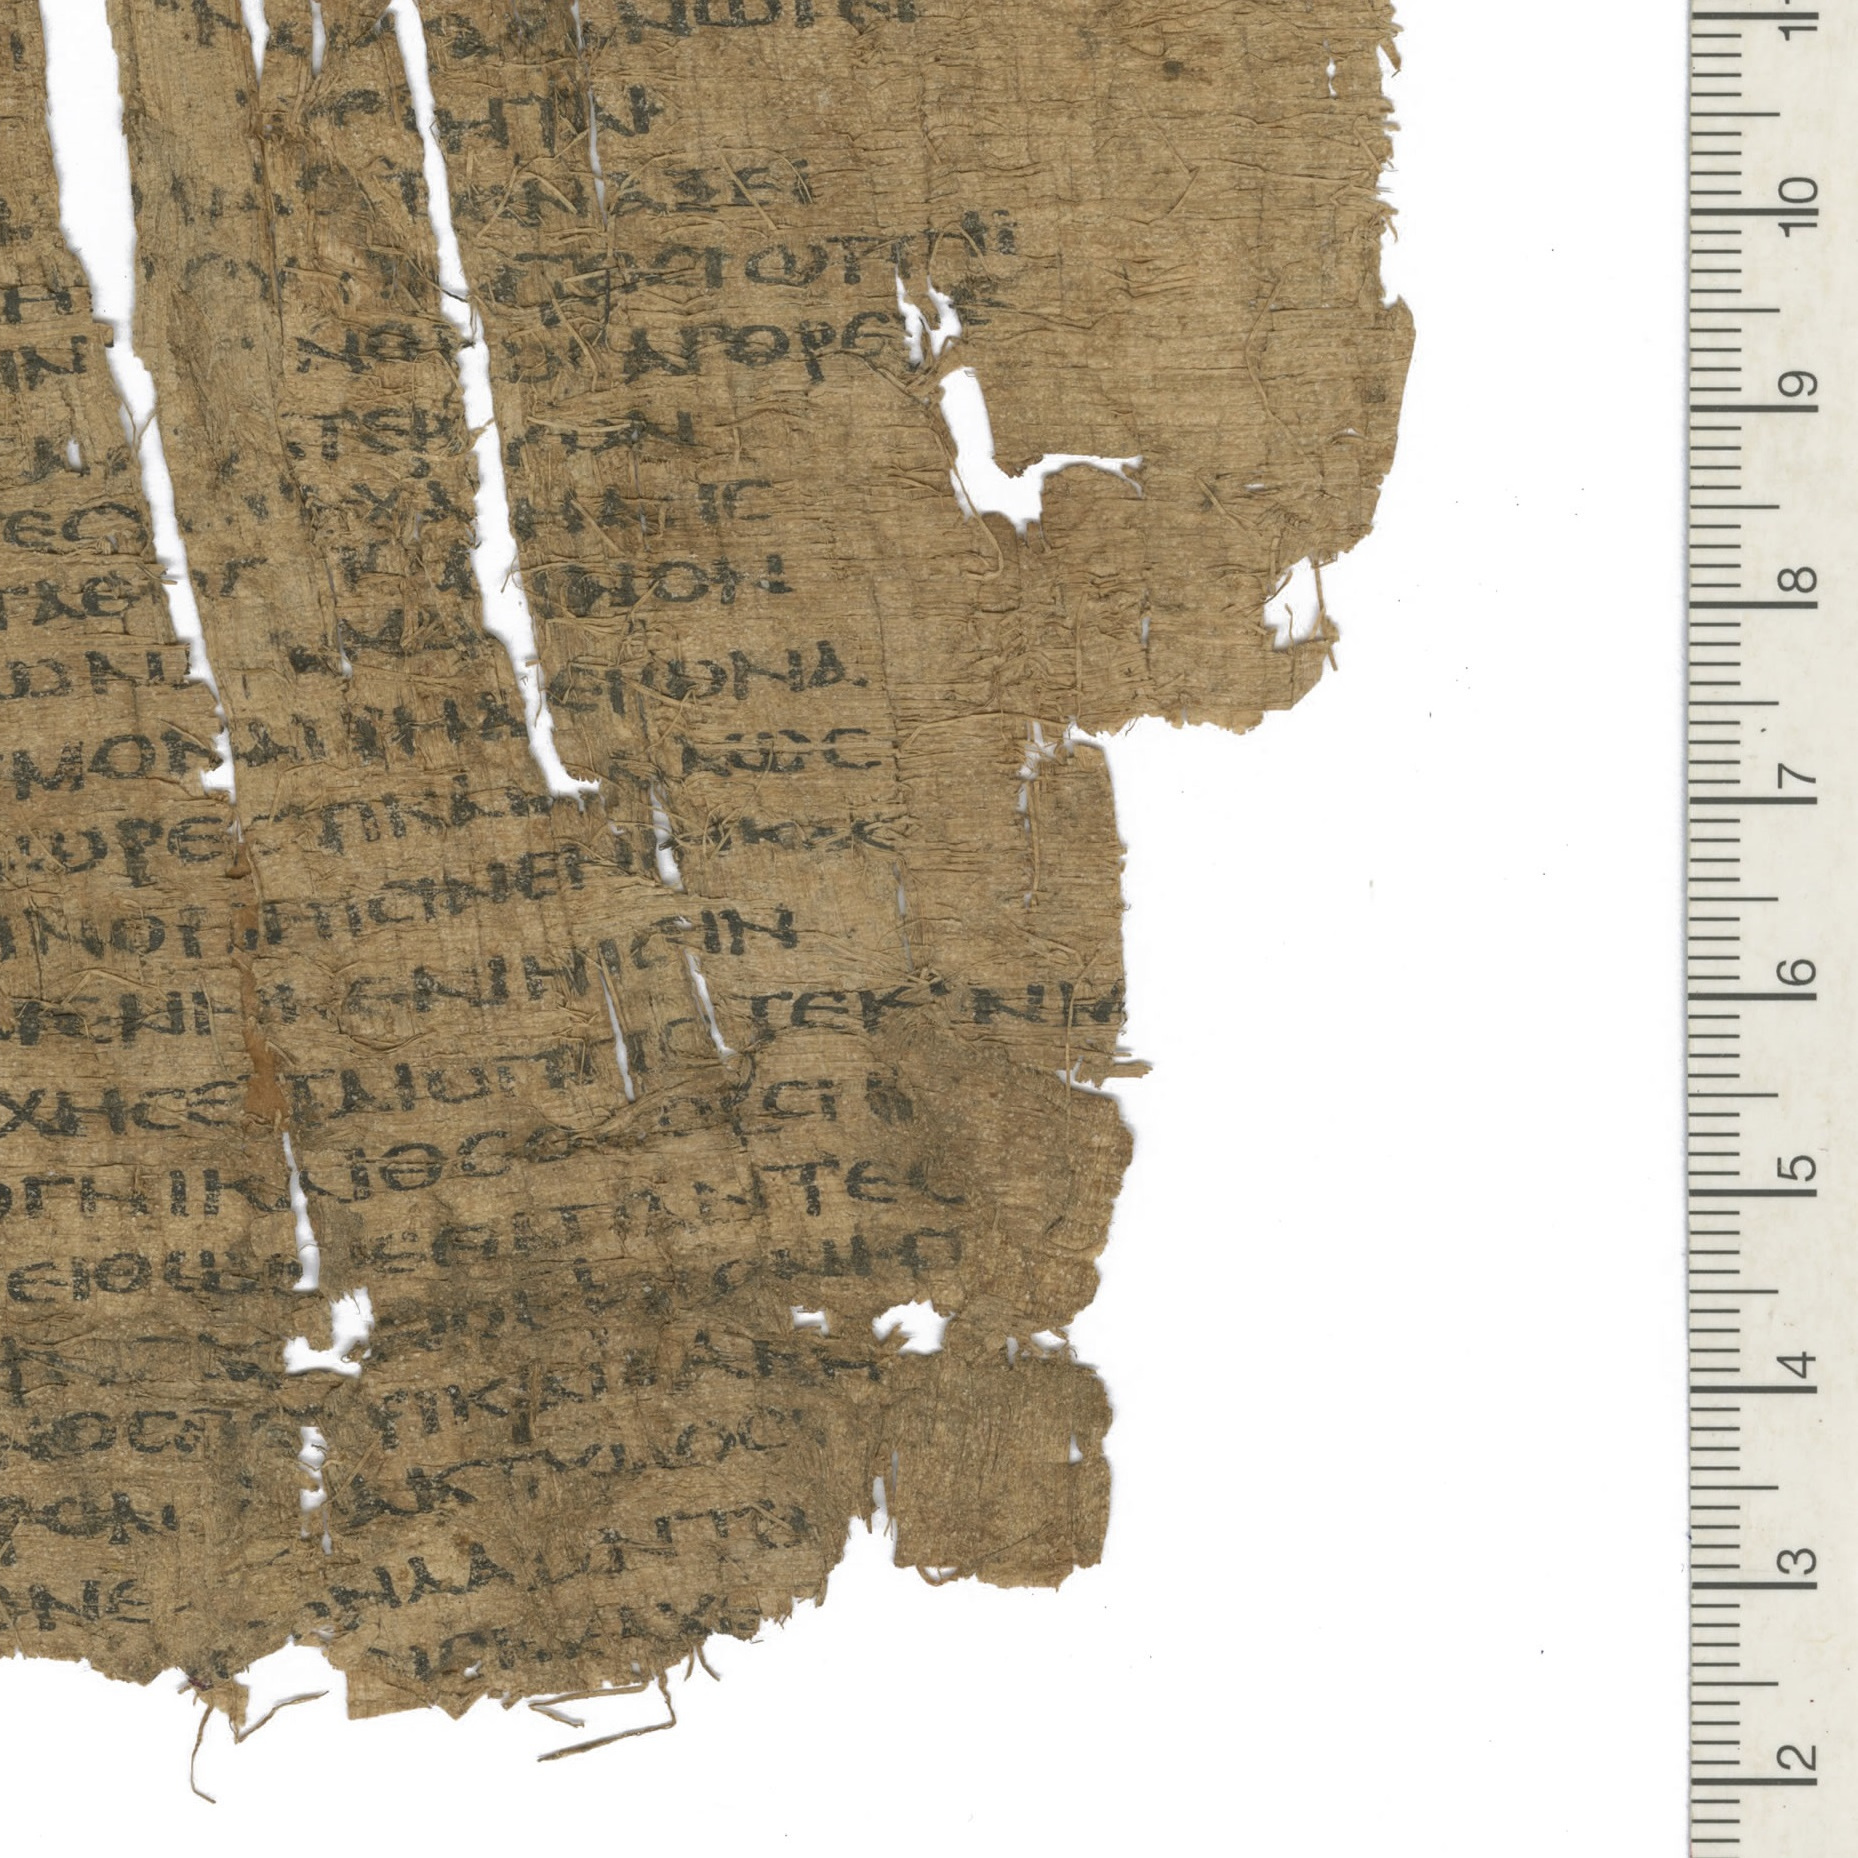
\includegraphics[width=\textwidth]{{raw/PSI_XIV_1377r_crop.jpg}}
        \end{subfigure}
    \end{center}
    The four images used to assess binarization methods, cropped to squares so that are easy to tile to make it easy to assess visually.
\end{figure}

\subsection{Evaluation of Methods}
\todo{NEW}

The results of k-means clustering on the evaluation images are included for reference \seefig{binarizationClustering}. These images clearly show that the signal to noise ratio is far too high to be utilized as the general binarization solution for the pipeline, as the signal to noise ratio is sometimes less than $1$.

The results generated by clustering can be directly compared to those of a neural network to see how poor they are. The results generated by DP-Linknet \seefig{binarizationCNN} are visibly much better at including whole glyphs and less of the noise included in the image, especially the papyrus noise.

Using the results of the Gabor wavelet approximation \seefig{binarizationGabor}, a binary mask can be created \seefig{binarizationGaborBinary} using DP-Linknet. This works using the assumption that large amounts of noise in the binary images generated by DP-Linknet are due to intentionally added objects in the original images, which are often more regular in color or shape than the glyphs, which means the Gabor filtered images do not lose this noise, allowing the CNN to pick up on this information to create an image that can be used as a mask to remove these details from the final binarizations \seefig{binarizationMaskedCNN}.

\begin{figure}
    \caption{Four Example Binarizations Generated with Clustering}
    \label{fig:binarizationClustering}
    \begin{center}
        \begin{subfigure}[b]{0.45\textwidth}
            \centering
            \caption{Example File A}
            
\includegraphics[width=\textwidth]{{binarization/clustering/G_02317_26742_Pap_crop.png}}
        \end{subfigure}
        \hfill
        \begin{subfigure}[b]{0.45\textwidth}
            \centering
            \caption{Example File B}
            \includegraphics[width=\textwidth]{{binarization/clustering/G_26734_c_crop.png}}
        \end{subfigure}
        \vfill
        \begin{subfigure}[b]{0.45\textwidth}
            \centering
            \caption{Example File C}
            \includegraphics[width=\textwidth]{{binarization/clustering/P_Hamb_graec_665_crop.png}}
        \end{subfigure}
        \hfill
        \begin{subfigure}[b]{0.45\textwidth}
            \centering
            \caption{Example File D}
            \includegraphics[width=\textwidth]{{binarization/clustering/PSI_XIV_1377r_crop.png}}
        \end{subfigure}
    \end{center}
    The four images were used to assess binarization methods, binarized using k-means with $k=5$. Image A has a near zero signal to noise ratio. Image B has a much better signal to noise ratio for the glyphs, but also contains text that should not be included near the bottom of the image. Images C and D also contain glyph signal, but are both noisy around the glyphs and include non-glyph information such as a ruler in Image D and the border and color scale in image C.
\end{figure}

\begin{figure}
    \caption{Four Example Binarizations Generated with DP-Linknet}
    \label{fig:binarizationCNN}
    \begin{center}
        \begin{subfigure}[b]{0.45\textwidth}
            \centering
            \caption{Example File A}
            
\includegraphics[width=\textwidth]{{binarization/cnn/G_02317_26742_Pap_crop.png}}
        \end{subfigure}
        \hfill
        \begin{subfigure}[b]{0.45\textwidth}
            \centering
            \caption{Example File B}
            \includegraphics[width=\textwidth]{{binarization/cnn/G_26734_c_crop.png}}
        \end{subfigure}
        \vfill
        \begin{subfigure}[b]{0.45\textwidth}
            \centering
            \caption{Example File C}
            \includegraphics[width=\textwidth]{{binarization/cnn/P_Hamb_graec_665_crop.png}}
        \end{subfigure}
        \hfill
        \begin{subfigure}[b]{0.45\textwidth}
            \centering
            \caption{Example File D}
            \includegraphics[width=\textwidth]{{binarization/cnn/PSI_XIV_1377r_crop.png}}
        \end{subfigure}
    \end{center}
    The four images used to assess binarization methods, binarized using DP-Linknet \cite{Xiong} with  confidence value of 2. Image A has clearly defined glyphs, especially when compared to the results of clustering. Image B has a similar signal to noise ratio for the glyphs to the clustering, with the extra text near the bottom of the image still being included. Images C and D also contain glyph signal, and are less noisy around the glyphs and include non-glyph information such as a ruler in Image D and the border and color scale in image C.
\end{figure}

\begin{figure}
    \caption{Four Example Gabor Filtered Images}
    \label{fig:binarizationGabor}
    \begin{center}
        \begin{subfigure}[b]{0.45\textwidth}
            \centering
            \caption{Example File A}
            
\includegraphics[width=\textwidth]{{binarization/gabor/G_02317_26742_Pap_crop.png}}
        \end{subfigure}
        \hfill
        \begin{subfigure}[b]{0.45\textwidth}
            \centering
            \caption{Example File B}
            \includegraphics[width=\textwidth]{{binarization/gabor/G_26734_c_crop.png}}
        \end{subfigure}
        \vfill
        \begin{subfigure}[b]{0.45\textwidth}
            \centering
            \caption{Example File C}
            \includegraphics[width=\textwidth]{{binarization/gabor/P_Hamb_graec_665_crop.png}}
        \end{subfigure}
        \hfill
        \begin{subfigure}[b]{0.45\textwidth}
            \centering
            \caption{Example File D}
            \includegraphics[width=\textwidth]{{binarization/gabor/PSI_XIV_1377r_crop.png}}
        \end{subfigure}
    \end{center}
    The four images used to assess binarization methods, passed through the Gabor wavelet approximation function.
\end{figure}

\begin{figure}
    \caption{Four Example Gabor Wavelet Binarized Images}
    \label{fig:binarizationGaborBinary}
    \begin{center}
        \begin{subfigure}[b]{0.45\textwidth}
            \centering
            \caption{Example File A}
            
\includegraphics[width=\textwidth]{{binarization/gaborMask/G_02317_26742_Pap_crop.png}}
        \end{subfigure}
        \hfill
        \begin{subfigure}[b]{0.45\textwidth}
            \centering
            \caption{Example File B}
            \includegraphics[width=\textwidth]{{binarization/gaborMask/G_26734_c_crop.png}}
        \end{subfigure}
        \vfill
        \begin{subfigure}[b]{0.45\textwidth}
            \centering
            \caption{Example File C}
            \includegraphics[width=\textwidth]{{binarization/gaborMask/P_Hamb_graec_665_crop.png}}
        \end{subfigure}
        \hfill
        \begin{subfigure}[b]{0.45\textwidth}
            \centering
            \caption{Example File D}
            \includegraphics[width=\textwidth]{{binarization/gaborMask/PSI_XIV_1377r_crop.png}}
        \end{subfigure}
    \end{center}
    The four images used to assess binarization methods, passed through the Gabor wavelet approximation function and then passed through DP-Linknet to create a rudimentary mask that contains some non-glyph information.
\end{figure}

\begin{figure}
    \caption{Four Example CNN Binarized Images (Masked)}
    \label{fig:binarizationGaborBinary}
    \begin{center}
        \begin{subfigure}[b]{0.45\textwidth}
            \centering
            \caption{Example File A}
            
\includegraphics[width=\textwidth]{{binarization/cnnMasked/G_02317_26742_Pap_crop.png}}
        \end{subfigure}
        \hfill
        \begin{subfigure}[b]{0.45\textwidth}
            \centering
            \caption{Example File B}
            \includegraphics[width=\textwidth]{{binarization/cnnMasked/G_26734_c_crop.png}}
        \end{subfigure}
        \vfill
        \begin{subfigure}[b]{0.45\textwidth}
            \centering
            \caption{Example File C}
            \includegraphics[width=\textwidth]{{binarization/cnnMasked/P_Hamb_graec_665_crop.png}}
        \end{subfigure}
        \hfill
        \begin{subfigure}[b]{0.45\textwidth}
            \centering
            \caption{Example File D}
            \includegraphics[width=\textwidth]{{binarization/cnnMasked/PSI_XIV_1377r_crop.png}}
        \end{subfigure}
    \end{center}
    The four images used to assess binarization methods, binarized using DP-Linknet \cite{Xiong} with  confidence value of 2 and then masked by the binarizations of the Gabor filtered images with the removed black parts of the image shown in grey. No changes were made to image A, as there was no detail that the CNN could recognize left in the Gabor filtered image. The extra text from image B is mostly removed, with the glyph information intact. Similarly, images C and D have their glyph information intact, with the artificial noise in the image being partially removed.
\end{figure}

% \subsection{BiNet}
% \todo{TODO: ADD CONTENT}

\section{Glyph Bounding}

\subsection{Evaluation Metrics}
\todo{NEW}

As the ground-truth information provided for bounding boxes are not tight, perfectly accurate metrics on bounding are not possible without manually tightly rebounding each glyph. Therefore, IOU is used, along with glyph precision and recall measuring the approximate efficacy of methods, with the caveat that a method may have a lower IOU if it generates tighter bounding boxes than if the bounding box was less tight.

Precision and recall are measured not on pixels, but on glyphs, where a prediction is considered to match a truth bounding box if the IOU between the two bounding boxes is greater than zero and each truth bounding box is paired with the prediction bounding box with the highest IOU value.

\subsection{Connected Components}
\todo{TODO: Nov 29}

\subsection{Region Based Convolution Neural Networks}
\todo{TODO: Nov 29}

\subsection{Sliding Window Region Based Convolution Neural Networks}
\todo{TODO: Nov 29}

\subsubsection{RCCN Sliding Window}
\todo{TODO: Nov 29}

\subsubsection{RCNN Duplicate Removal}
\todo{TODO: Nov 29}

\subsubsection{Binarization-Assisted CNN}
\todo{TODO: Nov 29}

\section{Line Bounding}
\todo{NEW}

As in glyph bounding, no ground truth information was provided for which glyphs where in the same line, so a visual approximation must be used to determine which methods are best, at least when comparing results of each metric without taking the rest of the pipeline into account.

\subsection{Point Of Interest Clustering}
\todo{TODO: : Nov 30}

\subsection{Point Of Interest Clustering}
\todo{TODO: : Nov 30}

\subsection{Adjacent Glyph Clustering}
\todo{TODO: : Nov 30}

\subsection{Overlaping Glyph Clustering}
\todo{TODO: : Nov 30}


\section{Classification}

\subsection{Transfer Learning}
\todo{TODO: ADD CONTENT}

\subsection{Convolutional Neural Networks}
\todo{TODO: ADD CONTENT}

\subsection{Stochastic Language Models}
\todo{TODO: ADD CONTENT}

\subsection{Neural Netork Language Models}
\todo{TODO: ADD CONTENT}


\section{Evaluation Metric Analysis}

\subsection{Ground Truth Comparison}
\todo{TODO: ADD CONTENT}

\subsection{Visual Analysis}
\todo{TODO: ADD CONTENT}

\subsection{BLEU Score}
\cite{Callison-Burch}
